\usetikzlibrary{calc,positioning}
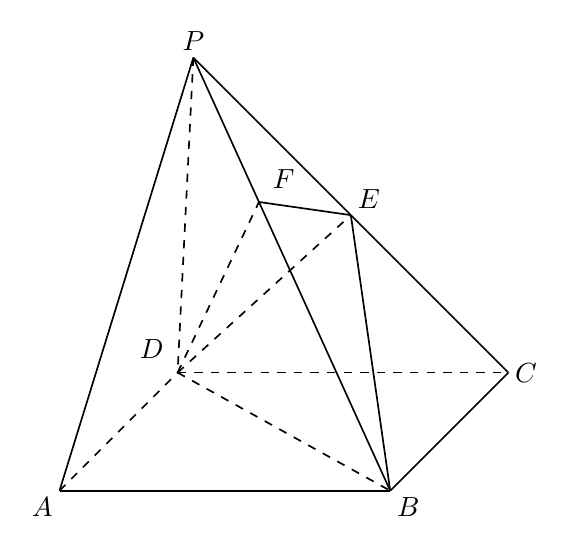
\begin{tikzpicture}[x=1cm,y=1cm,line width=.6pt,font=\normalsize,
 geometry edge/.style={solid,line width=.6pt,draw=black},
 geometry label/.style={font=\normalsize,inner sep=1.5pt,outer sep=1pt,draw=none}]

\coordinate (P) at (2,5.5);
\coordinate (D) at (1.8,1.5);
\coordinate (A) at (0.3,0);
\coordinate (B) at (4.5,0);
\coordinate (C) at (6,1.5);
\coordinate (E) at (4.0,3.5);
\coordinate (F) at (2.833333333,3.666666667);
\draw[geometry edge] (P)--(A);
\draw[geometry edge] (P)--(E);
\draw[geometry edge] (E)--(C);
\draw[geometry edge] (P)--(B);
\draw[geometry edge] (A)--(B);
\draw[geometry edge] (B)--(C);
\draw[geometry edge] (E)--(B);
\draw[geometry edge] (F)--(E);
\draw[geometry edge,dashed] (P)--(D);
\draw[geometry edge,dashed] (A)--(D);
\draw[geometry edge,dashed] (D)--(B);
\draw[geometry edge,dashed] (D)--(E);
\draw[geometry edge,dashed] (D)--(C);
\draw[geometry edge,dashed] (D)--(F);
\node[geometry label,above] at (P) {$P$};
\node[above left=2pt] at (D) {$D$};
\node[geometry label,below left] at (A) {$A$};
\node[geometry label,below right] at (B) {$B$};
\node[geometry label,right] at (C) {$C$};
\node[geometry label,above right] at (E) {$E$};
\node[above right=2pt] at (F) {$F$};
\end{tikzpicture}
